\chapter{Weather Research and Forecast (WRF)}
\section{Aspectos Generales}
El software ARW-WRF\footnote{Este capítulo es en gran parte una adaptación al español de la nota técnica del código WRF de \cite{https://doi.org/10.5065/d68s4mvh}. } (Advanced Research WRF) es un modelo atmosférico no hidrostático que resuelve las ecuaciones de Euler para flujo compresible en su forma conservativa y utilizando una coordenada vertical de masa (o de presión hidrostática). Su coordenada vertical se define como:
\begin{equation}\label{eq:04_eta}
\eta = \frac{p_{dh}-p_{dht}}{\mu_d},
\end{equation}
donde $p_{dh}$ corresponde a la componente hidrostática de la presión del aire seco, y:
\begin{equation}
\mu_d = p_{dhs} - p_{dht},
\end{equation}
es el peso de la columna del aire seco en la superficie. En estas ecuaciones los subíndices $t$ y $s$ corresponden a los límites superior (top) e inferior (surface) del dominio. Un esquema de cómo se distribuye esta coordenada verticalmente y cómo la malla sigue al terreno se presenta en la Figura \ref{fig:04_eta}.

\begin{figure}[h!]
	\centering
	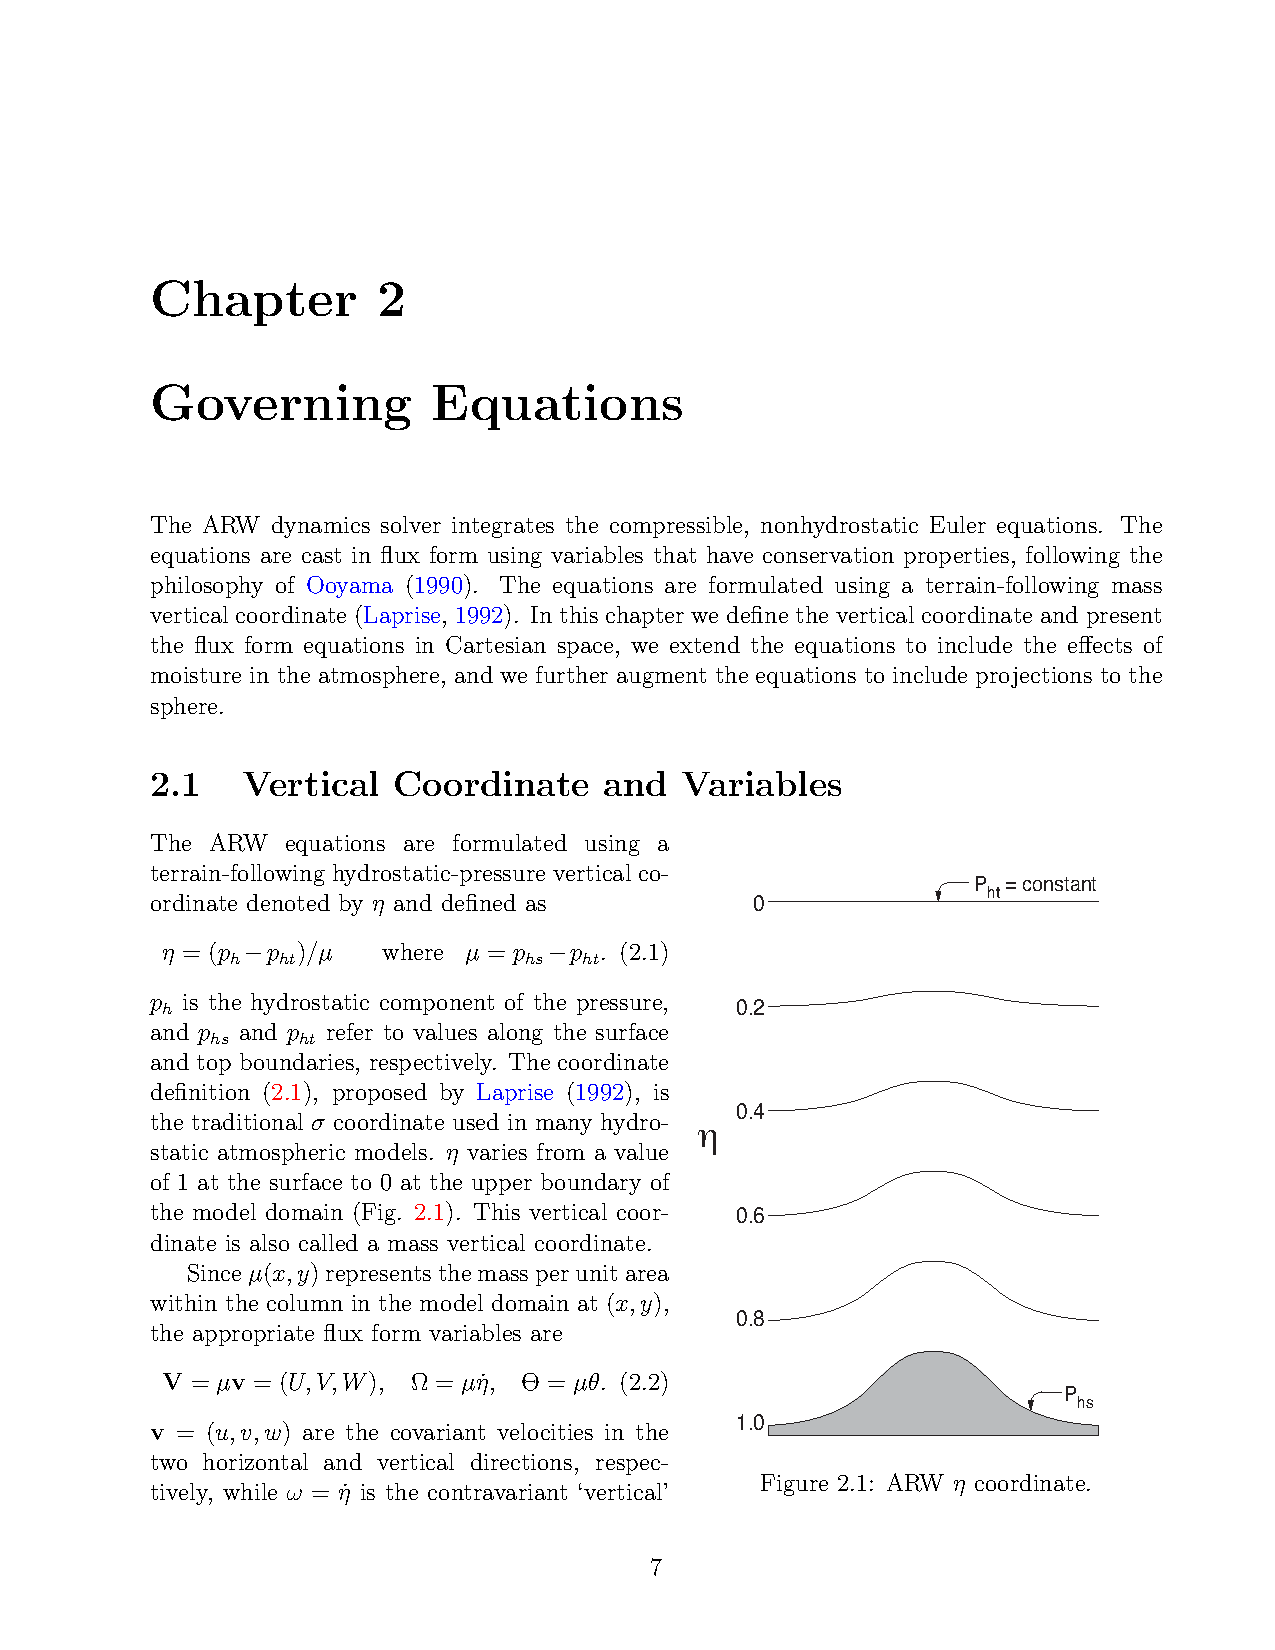
\includegraphics[width=0.55\linewidth,trim={11.5cm 3.3cm 1cm 14cm},clip]{Imagenes/04/eta}
	\caption{Estructura de la coordenada vertical. Fuente: \cite{https://doi.org/10.5065/d68s4mvh}.}
	\label{fig:04_eta}
\end{figure}

Las variables principales que resuelve WRF son las velocidades covariantes $(u,v,w)$, la masa de aire seco $\mu_d$, el geopotencial $\phi = gz$, la temperatura potencial $\theta$, la presión $p$, el inverso de la densidad $\alpha= 1/\rho$ y la energía cinética turbulenta $k$. 

El cambio de coordenadas que introduce la ecuación \ref{eq:04_eta} en las ecuaciones de Euler hace que aparezcan términos métricos y que la forma de escribir las ecuaciones sea diferente a lo acostumbrado a ver en mecánica de fluidos. El detalle de la transformación y el uso de $\mu_d$ en la ecuaciones se puede ver en la nota técnica del código \citep{https://doi.org/10.5065/d68s4mvh}.

A priori, las ecuaciones de momentum, temperatura potencial, energía cinética turbulenta y otros escalares relevantes tienen una forma acoplada con la masa de aire seco, de la forma:
\begin{equation}\label{eq:ec_conervacion}
\partial_t (\mu_d\theta) + \partial_x(\mu_d u \theta)+\partial_y(\mu_d v \theta)+\partial_\eta (\mu_d \omega \theta) = F.
\end{equation}
Si bien $\theta$ es la temperatura potencial, esta ecuación es válida para cualquier otro escalar mencionado anteriormente.
$F$ es la suma de los forzamientos externos (es una ecuación de Euler), como puede ser la mezcla turbulenta o fuerzas de Coriolis. Además:
\begin{equation}
\omega = d_t\eta = \dot{\eta},
\end{equation}
es la velocidad en la coordenada vertical. Notar que la ecuación \ref{eq:ec_conervacion} corresponde a una ecuación de conservación de un escalar pasivo.

Para la discretización espacial del modelo se utiliza una malla de Arakawa tipo C con un tamaño de malla constante en las direcciones horizontales, pero variable en la dirección vertical. Para la discretización temporal se utiliza un método explícito RK3 y un filtro que permite separar las ondas de alta frecuencia (ondas de presión y gravedad) de las ondas del espacio físico (o meteorológicamente relevantes). Las ondas de alta frecuencia son integradas en un paso de tiempo intermedio para asegurar estabilidad numérica.

A continuación se presenta una lista con las principales características del modelo ARW-WRF en su versión 3:
\begin{itemize*}
	\item Ecuaciones no hidrostáticas completamente compresibles (con opción hidrostática).
	\item Aplicaciones globales y regionales.
	\item Términos de transformación de curvatura y Coriolis completos.
	\item Código portátil capaz de correr en paralelo y en una gran variedad de sistemas operativos.
	\item Anidamiento de dos vías con múltiples nidos y niveles.
	\item Anidamiento de una vía con refinamiento vertical.
	\item Coordenada vertical basada en masa que se conforma al terreno.
	\item Espaciamiento vertical variable y ajustable.
	\item Factores de escala para proyecciones cartográficas: Conformal, Lambert, Mercator, Lat-Lon.
	\item Malla escalonada tipo Arakawa C.
	\item Integración temporal con métodos RK de 2do o 3er orden.
	\item Forma conservativa para las variables pronosticas.
	\item Opciones de advección (horizontal y vertical) de 2do hasta 6to orden.
	\item Opciones de transporte monótono y advección positiva para escalares.
	\item Formulación para la turbulencia de submalla en el espacio coordenado y físico.
	\item Filtro de amortiguamiento para la divergencia.
	\item Amortiguamiento de Rayleigh y absorción de ondas en el borde superior.
	\item Condiciones de borde laterales reales o ideales.
	\item Opciones para parametrización física de: capa superficial, capa límite planetaria, radiación superficial y atmosférica, microfísicas y convección de cúmulos.
	\item Modelos oceánicos.
	\item Incorporación de datos a través asimilación de datos.
	\item Inicialización con filtro digital.
	\item Paso de tiempo adaptativo.
	\item Ejemplos para casos idealizados.
\end{itemize*}

El desarrollo del modelo WRF ha sido un esfuerzo colaborativo entre NCAR (\emph{National Center for Atmospheric Research}), NOAA (\emph{National Oceanic and Atmospheric Administration}), NCEP (\emph{National Centers for Environmental Prediction}), ESRL (\emph{Earth System Research Laboratory}), NRL (\emph{Naval Research Laboratory}), AFWA (\emph{Department of Defense's Air Force Weather Agency}), CAPS (\emph{Center for Analysis and Prediction of Storms}), la universidad de Oklahoma y el FAA (\emph{Federal Aviation Administration}) con el objetivo de crear un modelo de predicción mesoescala de última generación para avanzar en la comprensión y predicción del clima, junto con entregar una herramienta de acceso libre a toda la comunidad.

Junto con el núcleo dinámico (ARW), el software WRF viene con un sistema de preproceso (WPS) que se encarga de formar los dominios, asignar las bases de datos de orografía y uso de suelo e interpolar horizontalmente las condiciones iniciales y de borde que se utilizarán. También, WRF viene con un código de asimilación de datos nativo (WRFDA) el cual es el encargado de manipular los datos de observaciones en terreno, filtrarlos y efectuar la asimilación de datos, habitualmente aplicado para mallas de macro y mesoescala.
 
\newpage
\section{Ecuaciones Resueltas}
Tal como se mencionó en la sección anterior, las ecuaciones a resolver serán las ecuaciones de Euler, las cuales, a priori, tienen una forma como la de la ecuación demostrativa \ref{eq:ec_conervacion} en el sentido de que la suma de las aceleración local y la aceleración advectiva se va a balancear con distintos forzamientos externos.

Para construir el sistema de ecuaciones que utiliza el solver, se deben considerar las siguientes modificaciones:
\paragraph{Coordenada Vertical} La descripción del sistema en función de la masa de aire seco $\mu_d$ introduce las siguientes variables acopladas:
\begin{equation}
\vec{V}=\mu_d\vec{v}=(U,V,W)\quad;\quad \Omega = \mu_d \omega \quad;\quad \Theta = \mu_d \theta
\end{equation}
De esta manera los operadores con los cuales es posible escribir las ecuaciones en forma conservativa quedan:
\begin{equation}
\nabla\cdot\vec{V}a = \partial_x(Ua)+\partial_y(Va)+\partial_\eta (\Omega a),
\end{equation}
\begin{equation}
\vec{V}\cdot \nabla a = U\partial_x a + V\partial_y a + \Omega\partial_\eta a.
\end{equation}
\paragraph{Inclusión de la Humedad} En vez de agregar términos fuentes a la ecuación de Euler, se trabaja considerando la conservación de masa del aire seco. Se agregan ecuaciones de conservación para las razones de mezcla $q_m=q_v,q_c,q_i,...$ que corresponden al vapor de agua, nubes, lluvia, hielo, etc. El valor de $\alpha$ para un elemento diferencial de aire se computa entonces como:
\begin{equation}
\alpha = \alpha_d(1+q_v+q_c+q_r+q_i+...),
\end{equation}
donde $\alpha_d$ es el volumen específico para aire seco.

La ecuación de estado ahora contempla la humedad de la siguiente forma:
\begin{equation}\label{eq:04_gasideal}
p = p_0\left(\frac{R_d \theta_m}{p_0 \alpha_d}\right)^\gamma,
\end{equation}
donde $R_d$ es la constante de gas ideal para el aire seco y $\gamma = c_p/c_v = 1.4$. Además:
\begin{equation}
\theta_m = \theta(1+(R_v/R_d)q_v)\approx\theta(1+0.61q_v),
\end{equation}
es la temperatura potencial virtual.
\paragraph{Proyecciones Cartográficas} Para implementar las proyecciones cartográficas, el ARW utiliza factores de mapa $m_x,m_y$. Estos corresponden a la razón entre una distancia en el espacio computacional y la misma distancia en la superficie de la tierra:
\begin{equation}
(m_x,m_y) = \frac{(\Delta x, \Delta y)}{\text{distancia en la tierra}}.
\end{equation}
De esta manera las variables de momentum quedan como:
\begin{equation}
U = \frac{\mu_d}{m_x}u\quad;\quad V = \frac{\mu_d}{m_y}v\quad;\quad W = \frac{\mu_d}{m_y}w\quad;\quad \Omega = \frac{\mu_d}{m_y}\dot{\eta}
\end{equation}
Si se utiliza una proyección isotrópica (Lambert conformal, Estereográfica polar, Mercator), los factores de mapa son idénticos: $m_x=m_y = m$.
\paragraph{Fuerza de Coriolis y Términos de Curvatura} Estos se agregan como forzamientos al lado derecho de la ecuación, tal como se muestra en la ecuación demostrativa \ref{eq:ec_conervacion}. Para el solver, estos toman la siguiente forma:
\begin{equation}
F_{U_{cor}} = \frac{m_x}{m_y}\left[ fV + \frac{uV}{a}\tan\psi \right] - \frac{uW}{r_e} - eW\cos\alpha_r,
\end{equation}
\begin{equation}
F_{V_{cor}} = \frac{m_y}{m_x}\left[ -fU + \frac{uU}{a}\tan\psi - \frac{vW}{r_e} - eW\sin\alpha_r \right],
\end{equation}
\begin{equation}
F_{W_{cor}} = e\left( U\cos\alpha_r - (m_x/m_y)V\sin\alpha_r \right) + \left( \frac{uU + (m_x/m_y)vV}{a} \right),
\end{equation}
donde $\alpha_r$ es el ángulo de rotación local entre el eje $y$ y los meridianos, $\psi$ es la latitud, $f=2\Omega_e\sin\psi, e=2\Omega_e\cos\psi$, $\Omega_e$ es la velocidad angular de la tierra y $a$ es el radio de la tierra.
\paragraph{Forma de Perturbación de las Ecuaciones Governantes} Finalmente, para disminuir los errores de truncatura, redondeo y otros problemas computacionales, se separan las variables de estado como la suma de una componente hidrostática (denotado por una barra superior) y una perturbación (denotado por una tilde).
\begin{equation*}
p=\overline{p}(\overline{z}) + p';\quad \phi=\overline{\phi}(\overline{z}) + \phi';\quad \alpha=\overline{\alpha}_d(\overline{z}) + \alpha_d';\quad \mu_d=\overline{\mu}_d(x,y) + \mu_d'
\end{equation*}

\newpage
De esta manera las ecuaciones \ref{eq:04_wrf1} -- \ref{eq:04_wrf2} son las que se utilizan en el solver.
\begin{equation}\begin{split}\label{eq:04_wrf1}
&\partial_t U + m_x[\partial_x(Uu)+\partial_y(Vu)]+\partial_\eta(\Omega u) \\
&+ (m_x/m_y)(\alpha/\alpha_d)[\mu_d(\partial_x\phi' + \alpha_d \partial_x p' + \alpha_d'\partial_x \overline p)+\partial_x\phi(\partial_\eta p' - \mu_d')] = F_U
\end{split}\end{equation}
\begin{equation}\begin{split}
&\partial_t V + m_y[\partial_x(Uv)+\partial_y(Vv)]+(m_y/m_x)\partial_\eta(\Omega v) \\
&+ (m_y/m_x)(\alpha/\alpha_d)[\mu_d(\partial_y\phi' + \alpha_d \partial_y p' + \alpha_d'\partial_y \overline p)+\partial_y\phi(\partial_\eta p' - \mu_d')] = F_V
\end{split}\end{equation}
\begin{equation}\begin{split}
\partial_t W + m_x[\partial_x(&Uw)+\partial_y(Vw)]+\partial_\eta(\Omega w) \\
\hspace{1cm}&- m_y^{-1}g(\alpha/\alpha_d)[\partial_\eta p' - \overline{\mu}_d(q_v+q_c+q_r)]+m_y^{-1}\mu_d' g = F_W
\end{split}\end{equation}
\begin{equation}\begin{split}
\partial_t \mu_d' + m_x m_y[\partial_x U + \partial_y V] + m_y\partial_\eta \Omega = 0
\end{split}\end{equation}
\begin{equation}\begin{split}
\partial_t \phi' + \mu_d^{-1}[m_x m_y(U\partial_x\phi + V\partial_y\phi) + m_y \Omega \partial_\eta\phi - m_ygW] = 0
\end{split}\end{equation}
\begin{equation}\begin{split}\label{eq:04_wrf2}
\partial_t \Theta + m_x m_y [\partial_x(U\theta)+\partial_y(V\theta)]+m_y\partial_\eta(\Omega \theta) = F_\Theta
\end{split}\end{equation}
Donde las primeras tres ecuaciones corresponden a la conservación de momentum, la cuarta a la conservación de masa, la quinta es la derivada material de la definición del geopotencial y la sexta es la ecuación de transporte para la temperatura potencial (o cualquier otro escalar relevante como las fracciones de mezcla de las fases del agua).

El sistema se cierra incorporando las ecuaciones diagnósticas para el geopotencial (en su forma de perturbación) y para la presión (gas ideal, ecuación \ref{eq:04_gasideal}):
\begin{equation}
\partial_\eta \phi ' = -\overline{\mu}_d \alpha_d' - \alpha_d \mu_d'.
\end{equation}

\newpage
\section{Aspectos Numéricos Relevantes}
A continuación se presentan en detalle aquellos aspectos del código que son fundamentales para el entendimiento y el desarrollo de los experimentos numéricos realizados. Algunos temas, como por ejemplo el tratamiento de la advección, la aplicación de ciertos filtros para amortiguar ondas o el detalle de la integración temporal para los modos físicos y acústicos, fueron dejados voluntariamente de lado en beneficio de la extensión de este trabajo. Se recomienda al lector revisar la nota técnica del modelo \citep{https://doi.org/10.5065/d68s4mvh} si desea tener un conocimiento extensivo con respecto al funcionamiento integral del WRF.
\subsection{Difusión}
La difusión y los flujos turbulentos en el espacio físico $(x,y,z)$ se calculan haciendo uso de la métrica del espacio a partir de la ecuación para el geopotencial $\phi$:
\begin{eqnarray}
z_x=g^{-1}\delta_x\phi, \\
z_y=g^{-1}\delta_y\phi,
\end{eqnarray}
donde $\delta_{x,y}$ es el operador discreto para la derivada, es decir:
\begin{equation}
\delta_x a = \frac{a_{i+1/2}-a_{i-1/2}}{\Delta x}.
\end{equation}
El término difusivo se agrega al lado derecho de las ecuaciones de Euler, junto al resto de las fuerzas externas. Estas se presentan de la siguiente manera:
\begin{eqnarray}
\partial_t U = \ldots - m_x[\partial_x\tau_{11}+\partial_y\tau_{12}-\partial_z(z_x\tau_{11}+z_y\tau_{12})]-\partial_z\tau_{13}, \\
\partial_t V = \ldots - m_y[\partial_x\tau_{12}+\partial_y\tau_{22}-\partial_z(z_x\tau_{12}+z_y\tau_{22})]-\partial_z\tau_{23}, \\
\partial_t W = \ldots - m_y[\partial_x\tau_{13}+\partial_y\tau_{23}-\partial_z(z_x\tau_{13}+z_y\tau_{23})]-\partial_z\tau_{33},
\end{eqnarray}
Y el tensor de esfuerzos viscosos es:
\begin{equation}
\tau_{ij} = -\mu_d K_{h,v}S_{ij},
\end{equation}
donde $K_{h,v}$ es la viscosidad turbulenta en dirección horizontal o vertical según corresponda y $S_{ij}$ es el tensor tasa de deformación que bajo esta formulación toma la siguiente forma:
\begin{align}
S_{11} &= 2m_xm_y[\partial_x(m_y^{-1}u)-z_x\partial_z(m_y^{-1}u)],  \\
S_{22} &= 2m_xm_y[\partial_y(m_x^{-1}v)-z_y\partial_z(m_x^{-1}v)],  \\
S_{33} &= 2\partial_z w,  \\
S_{12} &= m_xm_y[\partial_y(m_y^{-1}u)-z_y\partial_z(m_y^{-1}u)+\partial_x(m_x^{-1}v)-z_x\partial_z(m_x^{-1}v)],  \\
S_{13} &= m_xm_y[\partial_x(m_y^{-1}w)-z_x\partial_z(m_y^{-1}w)]+\partial_z u,  \\
S_{23} &= m_xm_y[\partial_y(m_y^{-1}w)-z_y\partial_z(m_y^{-1}w)]+\partial_z v,  \\%
\end{align}

Por otro lado, la difusión de un escalar cualquiera $a$ es:
\begin{equation}\begin{split}
\partial_t(\mu_d a) = ... &+ [m_x(\partial_x-\partial_z z_x)(\mu_d m_x K_h(\partial_x - z_x\partial_z)) \\
&+m_y(\partial_y-\partial_z z_y)(\mu_d m_y K_h(\partial_y-z_y\partial_z))+\partial_z\mu_dK_v\partial_z]a.
\end{split}\end{equation}

\subsubsection{Cálculo de la Viscosidad Turbulenta}
La opción por defecto para el modelo (simulaciones de mesoescala sin LES), es computar la viscosidad turbulenta horizontal $K_h$ por medio de la deformación horizontal usando un esquema de Smagorinsky de primer orden,
\begin{equation}
K_h = C_s^2 l^2[0.25(D_{11}-D_{22})^2+D_{12}]^{0.5}.
\end{equation}
Con $C_s=0.25$ y $l=\sqrt{\Delta x\Delta y}$. La viscosidad turbulenta vertical $K_v$ queda definida según el esquema de parametrización utilizado para la capa límite planetaria.

Para las simulaciones de microescala utilizando LES la viscosidad turbulenta se calcula en función de la energía cinética turbulenta $k$ de la forma:
\begin{equation}
K_{h,v}=C_k l_{h,v}\sqrt{k}.
\end{equation}
donde $C_k$ es una constante (normalmente $0.15<C_k<0.25$) y $l$ es un largo característico que se calcula en función de la isotropía de la malla, la resolución, $k$ y la estratificación térmica de la forma:
\begin{align}
	l_{h,v} &= \min[(\Delta x \Delta y \Delta z)^{1/3}, 0.76\sqrt{k}/N]\quad&;&\quad N^2>0\\
	l_{h,v} &= (\Delta x \Delta y \Delta z)^{1/3}\quad&;&\quad N^2\leq 0 
\end{align}
$N$ es la frecuencia de Brunt-Väisälä calculada para aire húmedo.

La clausura del modelo de turbulencia se hace considerando la ecuación de transporte para $k$ como:
\begin{equation}
\partial_t(\mu_d k) + (\nabla\cdot\vec{V}k)_\eta = \mu_d(\mathcal{P} + \mathcal{F} + \mathcal{D}).
\end{equation}
Los términos al lado derecho corresponden a la producción mecánica, a la producción por flotación y a la disipación de energía cinética turbulenta respectivamente. Estos se calculan como:
\begin{align}
	\mathcal{P}&= K_h (S_{11}^2 + S_{22}^2 + S_{12}^2) + K_v (S_{33}^2 + S_{13}^2 + S_{23}^2),\\
	\mathcal{F}&=-K_v N^2,\\
	\mathcal{D}&=-\frac{C k^{3/2}}{l_k},
\end{align}
Con las siguientes constantes:
\begin{align}
	C &= 1.9C_k + \frac{(0.93 - 1.9 C_k)l_k}{(\Delta x \Delta y \Delta z)^{1/3}},\\
	l_k &= \min[(\Delta x \Delta y \Delta z)^{1/3}, 0.76\sqrt{e}/N],
\end{align}
Así, queda entonces cerrado el problema de la turbulencia.

\subsection{Parametrizaciones Físicas}
Junto con el esquema para la difusión, el modelo ARW presenta otros esquemas disponibles para representar los fenómenos físicos que ocurren dentro de la atmósfera. Estos esquemas generalmente se presentan como \emph{drivers} independientes del código principal y por lo tanto son usados como librerías para actualizar las tendencias de las variables de estado que modelan las ecuaciones de Euler. Las categorías de las físicas parametrizadas son: (i) Microfísicas, (ii) Capa Límite Atmosférica, (iii) Modelo de suelo-superficie, (iv) Cúmulos y (v) Radiación.

A continuación se explicará brevemente la importancia dentro de la simulación de cada una, sin recurrir a desarrollos matemáticos extensos, debido a que WRF ofrece una gran variedad de opciones para cada una de las  parametrizaciones físicas.
\subsubsection{Microfísicas}
Se encarga de resolver explícitamente el vapor de agua, nubosidad y procesos de precipitación. También incluye procesos de sedimentación y el ajuste a la saturación. La diferencia entre los distintos modelos recae en la cantidad de variables a solucionar y el tipo de variables. Los modelos mas sofisticados pueden modelar 10 variables, incluyendo procesos de formación de hielo y variables con mezcla de fases.
\subsubsection{Parametrización de Cúmulos}
Son responsables de modelar el efecto de submalla de las nubes convectivas. En específico busca representar los flujos verticales debido a las escalas no resueltas y compensar el movimiento fuera de las nubes. Opera sobre toda una columna de aire y entrega el calentamiento vertical y perfiles de humedad. Los modelos más avanzados pueden entregar los campos de tendencias para nubes y precipitación.

Teóricamente, esta parametrización debe usarse solo para malla gruesas (>10 [km]) cuando es necesario representar el movimiento que no pudo ser resuelto. Mallas más finas pueden resolver explícitamente los vórtices verticales y por lo tanto no requiere usarse.
\subsubsection{Capa Superficial}
Los esquemas de capa superficial se encargan de calcular la velocidad de fricción $u^*$ y los coeficientes de mezcla que permiten el cálculo de los flujos de calor y humedad desde la superficie por el esquema de modelo de suelo y los esfuerzos de pared por el esquema de capa límite. Generalmente cada modelo de capa superficial tiene su modelo de capa límite asociado, sin embargo, se espera que en el futuro estos puedan independizarse. La manera de hallar los coeficientes se hace a través del uso de funciones de estabilidad o por teorías de similaridad como la propuesta por Monin-Obukhov.
\subsubsection{Modelo de Suelo}
A través de los resultados obtenidos por los modelos de capa superficial, microfísicas, cúmulos y radiación, junto con los datos sobre el uso de suelo del terreno, el modelo de suelo se encarga de calcular los flujos de calor y humedad desde el suelo hacia la atmósfera. Estos flujos proveen las condiciones de borde inferior para el transporte vertical hecho por el modelo de capa límite. Los modelos de suelo poseen un amplio espectro de sofisticación, pudiendo manejar flujos térmicos y de humedad en numerosas capas de la tierra, junto con vegetación, raíces, cobertura de nieve, etc. Este modelo no modifica las tendencias de las variables de estado, sino que actualiza las condiciones del suelo.
\subsubsection{Capa Límite Planetaria}
Se encarga de entregar los flujos verticales de submalla ($K_v$) debido al transporte turbulento para toda la columna de aire, no solo la capa límite y de esta manera actualiza las tendencias de temperatura, humedad y momentum horizontal para el modelo. La mayoría de los modelos considera mezcla seca para la capa límite, pero existen modelos mas avanzados que pueden manejar efectos de saturación para la estabilidad vertical. Este esquema es unidimensional y asume que existe una clara separación entre los vórtices de submalla y los vórtices resueltos (i.e. fuera de la zona gris de la turbulencia). A medida que la resolución de la malla va aumentando hasta el tamaño de los metros, es mejor no utilizar un modelo de capa límite y calcular explícitamente la mezcla vertical a través de un modelo 3D para la turbulencia (modo LES).
\subsubsection{Radiación Atmosférica}
Se encarga de calcular el calentamiento de la atmósfera debido a la divergencia del flujo radiativo y a la radiación de onda corta y onda larga desde la superficie. La radiación de onda larga incluye la radiación infrarroja o térmica absorbida y emitida por los gases y superficies, además del flujo radiativo emitido por la superficie. La radiación de onda corta incluye la radiación emitida por el sol dentro del espectro visible. Si bien la única fuente de onda corta es el sol, estos procesos incluyen la absorción, reflexión, y dispersión de las ondas en la atmósfera y superficies.

\newpage
\section{Sistema de Asimilación de Datos WRFDA}
Tal como se explicó en el marco teórico, la función que se busca minimizar es la siguiente:
\begin{equation}
J(x) = \frac{1}{2}(\mathbf{x}-\mathbf{x_b})^T\mathbf{B}^{-1}(\mathbf{x}-\mathbf{x_b}) + \frac{1}{2}(\mathbf{y}-H(\mathbf{x}))^T \mathbf{R}^{-1}(\mathbf{y}-H(\mathbf{x})).
\end{equation}
El modelo WRF efectúa esto a través de una formulación incremental del problema. Linealizando, sea $\delta \mathbf{x}=\mathbf{x} - \mathbf{x}_g$ y $\delta \mathbf{x}_g=\mathbf{x}_b - \mathbf{x}_g$ se tiene:
\begin{equation}
	J(\delta \mathbf{x}) = \frac{1}{2}(\delta \mathbf{x}- \delta \mathbf{x}_g)^T\mathbf{B}^{-1}(\delta \mathbf{x} - \delta \mathbf{x}_g) + \frac{1}{2}[H(\delta \mathbf{x} + \mathbf{x}_g)-\mathbf{y}]^T \mathbf{R}^{-1}[H(\delta \mathbf{x} + \mathbf{x}_g)-\mathbf{y}].
\end{equation}
Luego, se aplica una serie de Taylor para el término de las observaciones:
\begin{equation}
J(\delta \mathbf{x}) = \frac{1}{2}(\delta \mathbf{x}- \delta \mathbf{x}_g)^T\mathbf{B}^{-1}(\delta \mathbf{x} - \delta \mathbf{x}_g) + \frac{1}{2}(\mathbf{H} \delta \mathbf{x} -\textbf{d})^T \mathbf{R}^{-1}(\mathbf{H}\delta \mathbf{x} -\textbf{d}),
\end{equation}
donde $d=y-H(\textbf{x}_g )$ y $\textbf{H}$ es la versión linealizada de $H$ en las cercanías de $\textbf{x}_g$.

En esta formulación $\textbf{x}_g$ es el primer estimador de la solución. Para la primera iteración $\textbf{x}_b=\textbf{x}_g$, pero en las iteraciones siguientes $\textbf{x}_g$ será el análisis del ciclo anterior $\textbf{x}_a$.

Para evitar el cálculo de la inversa de la matriz $\textbf{B}$, se hace el siguiente cambio de variable a la variable de control $\textbf{v}$:
\begin{equation}
	\delta \mathbf{x}=\textbf{U}\textbf{v}\quad;\quad \delta \mathbf{x}_g=\textbf{U}\textbf{v}_g 
\end{equation}
Donde $\textbf{U}$ es la raíz cuadrada de $\textbf{B}$ (en el sentido matricial), es decir:
\begin{equation}
\textbf{B}=\textbf{B}^{1/2}\textbf{B}^{T/2} = \textbf{U}\textbf{U}^{T},
\end{equation}
o,
\begin{equation}
\textbf{U}=\textbf{B}^{1/2}.
\end{equation}
De la misma forma:
\begin{equation}
\textbf{B}^{-1} = \textbf{U}^{-T}\textbf{U}^{-1}.
\end{equation}
La función de costo con respecto a la variable de control $\textbf{v}$ se vuelve:
\begin{equation}
J(\mathbf{v}) = \frac{1}{2}(\mathbf{v}- \mathbf{v}_g)^T(\mathbf{v} - \mathbf{v}_g) + \frac{1}{2}(\mathbf{H} \mathbf{U}\mathbf{v} -\textbf{d})^T \mathbf{R}^{-1}(\mathbf{H}\mathbf{U}\mathbf{v} -\textbf{d}).
\end{equation}
\subsection{Modelación de $\textbf{B}$}
Tal como se explicó en el capítulo del marco teórico, la matriz de covarianzas del error del \emph{background} $\textbf{B}$ es la encargada de (a) ponderar correctamente el valor del \emph{background} al análisis, y (b) distribuir la información espacialmente y a través de todas las variables. WRF posee su propio mecanismo de generación de la matriz $\textbf{B}$ utilizando el llamado método NMC \citep{https://doi.org/10.5065/d68s4mvh}.

Algunas propiedades relevantes de la matriz son:
\begin{itemize*}
	\item $\textbf{B}$ es cuadrada y simétrica.
	\item $\textbf{B}$ es una matriz semidefinida positiva, es decir, sus valores propios son positivos. 
\end{itemize*}

En WRF esta matriz se forma a través de tres transformaciones secuenciales de la forma:
\be 
\textbf{B}=\textbf{U}_p \textbf{U}_v \textbf{U}_h \textbf{U}_p^T \textbf{U}_v^T \textbf{U}_h^T. 
\ee
Donde $\textbf{U}_h$ es la transformación horizontal a través de filtros recursivos para modelar la correlación horizontal de las variables de control, $\textbf{U}_v$ es la transformación vertical a través de una descomposición en funciones ortogonales de la varianza vertical y $\textbf{U}_p$ es la transformación de balance/física a través de regresiones lineales con la función de corriente.